\chapter{Hintergrundwissen}%
\label{cha:Hintergrundwissen}

\section{Konvexe Funktionen}%
\label{sec:Konvexe Funktionen}

\begin{definition}
\label{thm:konvexmenge}
	Eine Menge $X \subseteq \R^{n}$ heißt \underline{konvex} , wenn gilt
	\[
		\forall x,y \in X, \forall c \in [0,1] \colon 
		cx + (1-c)y \in X
	.\] 
\end{definition}

\begin{beispiel}
\label{thm:bspkonvexmenge}
Einige Beispiele

\begin{figure}[ht!]
	\begin{center}
		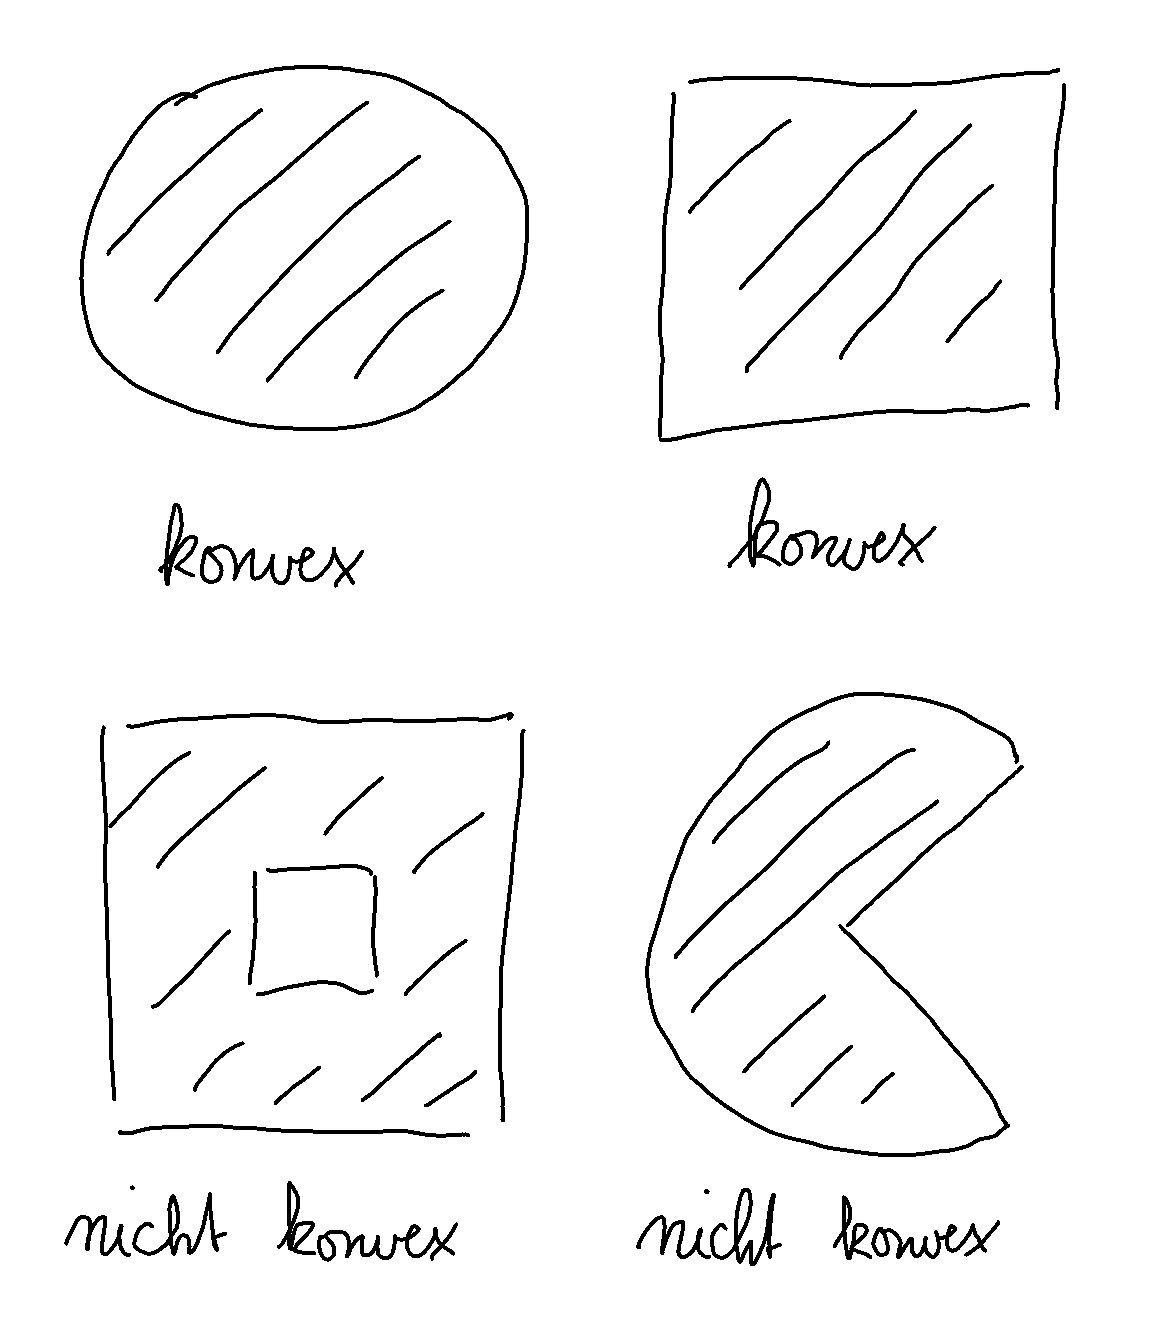
\includegraphics[width=0.5\textwidth]{pics/2.png}
	\end{center}
	\caption{Beispiele konvexer und nicht-konvexer Mengen}
	\label{fig:konvexemengen}
\end{figure}

\end{beispiel}

\begin{definition}
\label{thm:konvexfunktion}
	Sei $X \subseteq \R^{n}$ konvex. Dann heißt $f:X \rightarrow \R$
	\begin{enumerate}[label=\alph{enumi})]
		\item \underline{konvex} (auf $X$), wenn gilt
			\[
				\forall x,y \in X, \forall c \in [0,1] \colon f(cx + (1-c)y) \leq cf(x) + (1-c)f(y)
			.\] 
		\item \underline{strikt konvex} (auf $X$), wenn gilt
			\[
				\forall x,y \in X, x \neq y, \forall c \in (0,1) \colon f(cx + (1-c)y) < cf(x) + (1-c)f(y)
			.\] 
		\item \underline{gleichmäßig konvex} (auf $X$), wenn es ein $\mu>0$ gibt mit
			\[
				\forall x,y \in X, \forall c \in [0,1] \colon f(cx+ (1-c)y) \leq cf(x) + (1-c)f(y) - \mu c(1-c) \norm{x-y}^{2}
			.\] 
			\begin{figure}[ht!]
			\begin{center}
				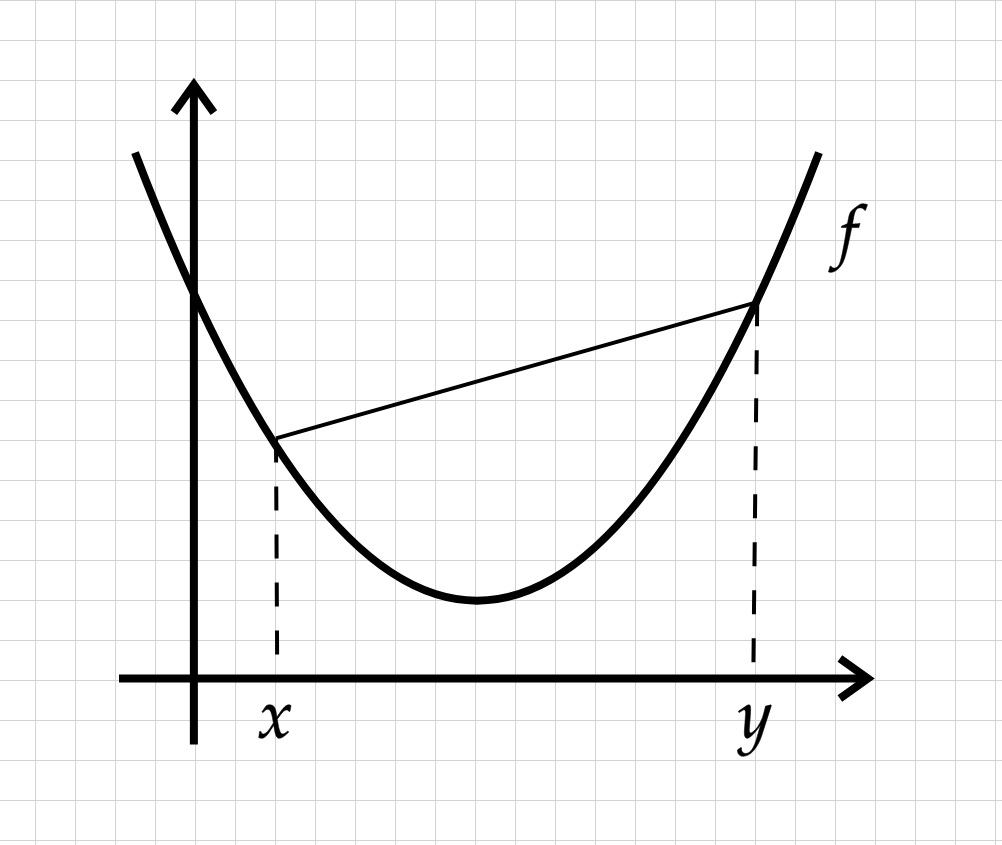
\includegraphics[width=0.4\textwidth]{pics/texplot1.png} 
				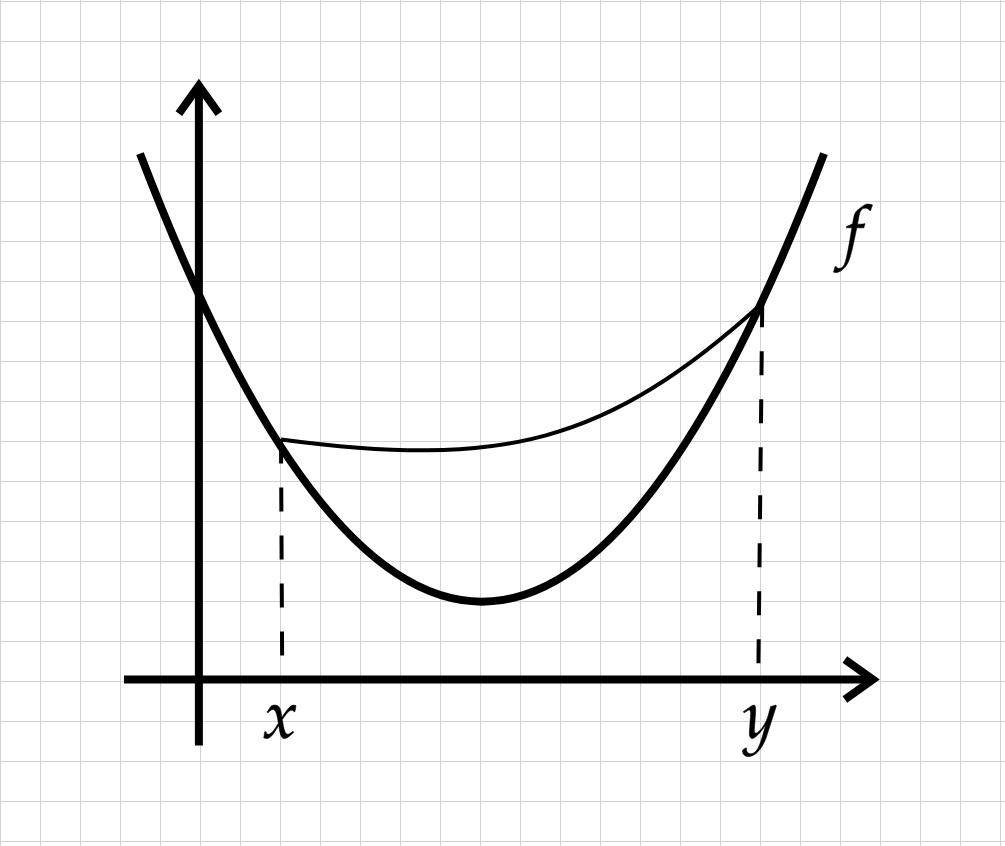
\includegraphics[width=0.4\textwidth]{pics/texplot2.png}
			\end{center}
			\caption{links: konvexe Funktion, rechts: glm. konvexe Funktion}
			\label{fig:glmkonvexefunktion}
			\end{figure}

			Man kann Konvexität in einfachen Fällen auch erkennen, dass gilt: "Jede Verbindungslinie zwischen zwei beliebigen Funktionswerten befindet sich überhalb des Graphen"
			
	\end{enumerate}
	Es gilt außerdem
	\[
	f \text{ glm. konvex} \implies f \text{ strikt konvex} \implies f \text{ konvex}
	.\] 
\end{definition}

\begin{beispiel}
\label{thm:bspkonvexfunktion1}

Einige Beispiele für konvexe Funktionen:
\begin{enumerate}[label=\alph{enumi})]
	\item $f$ konvex, aber nicht strikt konvex : $f(x)=c, f(x)=ax$
	\item $f$ strikt konvex, aber nicht glm. konvex : $f(x)=e^{x}, f(x)= x^{4}$
\end{enumerate}
\end{beispiel}

\begin{beispiel}
\label{thm:bspkonvexfunktion2}
Sei $f\colon \R^{n} \rightarrow \R$ mit 
\[
f(x) = \frac{1}{2}x^{T}Qx + c^{T}x+ \gamma
,\]

wobei $Q=Q^{T}$ (sonst $\tilde{Q}= \frac{1}{2}(Q+Q^{T})$). Dann gilt
\[
	cf(x)+(1-c)f(y) = f(cx+(1-c)y) + c(1-c)(x-y)^{T}Q(x-y)
\] 
und damit sieht man 
\begin{align*}
	f \text{ konvex auf } \R^{n} &\iff Q \text{ pos. semidef.} \\
	f \text{ strikt konvex auf } \R^{n} &\iff Q \text{ pos. def.} \iff f \text{ glm. konvex} \\
	Q \text{ pos. def. } &\implies c(1-c)(x-y)^{T}Q(x-y) \geq c(1-c)\norm{x-y} ^2 \underbrace{\lambda_{\min}(Q)}_{=:\mu} 
\end{align*}
\end{beispiel}

\begin{satz}
\label{thm:konvexcharakterisierung}
Sei $X \subseteq \R^{n}$ konvex und $f \colon X \rightarrow \R$ stetig differenzierbar. Dann gelten:
\begin{enumerate}[label=\alph{enumi})]
	\item $f$ konvex $\iff \forall x,y \in X \colon f(y) \geq f(x) + \nabla f(x)^{T}(y-x)$
	\item $f$ strikt konvex $\iff \forall x,y \in X, x \neq y \colon f(y) > f(x) + \nabla f(x)^{T}(y-x)$
	\item $f$ glm. konvex $\iff$ 
		\[
		\exists \mu > 0 \forall x,y \in X \colon f(y) \geq f(x) + \nabla f(x)^{T}(y-x) + \mu \norm{y-x} ^2
		.\]
\end{enumerate}
\end{satz}

\begin{proof}
\label{thm:konvexcharakterisierungbeweis}

\begin{itemize}[label=]
	Wir beweisen zunächst Fall (c), da der Rest schnell aus diesem Fall folgt.
	\item (c)
		\begin{itemize}[label=]
			\item "$\Leftarrow$"

 		Sei $\mu>0$, sodass 
		\[
		\forall x,y \in X \colon f(y)\geq f(x) + \nabla f(x)^{T}(y-x) + \mu \norm{x-y} ^2
		\] 
		erfüllt ist.

Seien $x,y \in X$ und $c \in [0,1]$ und $z = cx +(1-c)y$
\begin{align*}
	\implies & f(x) \geq f(z) + \nabla f(z)^{T}(x-z) + \mu \norm{x-z} ^2 \\
			 &f(y) \geq f(z) + \nabla f(z)^{T}(y-z) + \mu \norm{y-z} ^2 \\
	\overset{\text{Add.}}{\implies} &cf(x) + (1-c)f(y) \geq f(z) + \nabla f(z)^{T}[c(x-z) + (1-c)(y-z)] \\
									&\qquad\qquad\qquad\qquad\qquad+\underbrace{\mu c \norm{x-z} ^2 + \mu(1-c) \norm{y-z} ^2}_{2\mu c(1-c) \norm{x-y} ^2}  \\
	\implies &f \text{ glm. konvex.}
\end{align*}

\item "$\Rightarrow$"

	Sei $f$ glm. Konvex, d.h. $\exists \mu > 0, \forall x,y \in X, \forall c \in [0,1]$, sodass gilt
	\[
	f(cx+(1-c)y) \leq c(fx) + (1-c)f(y) - \mu  c(1-c) \norm{y-x} ^2
	.\] 
\begin{align*}
	\implies &f f(y+ c(x-y)) - f(y) \leq f(x) - f(y) - \mu (1-c)\norm{x-y}^2 \\
	\overset{c \downarrow 0}{\implies} & \nabla f(y)^{T}(x-y) \leq f(x) - f(y) - \mu \norm{x-y} ^2
\end{align*}
		\end{itemize}

	\item (a)

		analog zu (c) mit $\mu = 0$.

	\item (b)

		\begin{itemize}[label=]
			\item "$\Leftarrow$"

 $\mu=0$, $>$ statt $\geq$, $x \neq y$, $c \in(0,1)$ analog zu (c)

 \item "$\Rightarrow$"

 geht nicht völlig analog zu (c) wegen Grenzübergang $c \downarrow 0$.

 Sei $f$ strikt konvex und $x\neq y$, $x,y \in X$. Dann gilt durch (a):
\[
	f(z) \geq f(x) + \nabla f(x)^{T}(z-x)
\] 
$  \text{mit }z=\frac{1}{2}x + \frac{1}{2}y \text{ und } f(z) < \frac{1}{2}f(x) + \frac{1}{2}f(y)$ 

Und damit folgt
\[
	f(y) > f(x) + \nabla f(x)^{T}(x-y)
.\] 
	\end{itemize}
\end{itemize}

\end{proof}

\section*{Verallgemeinerungen von Konvexität}%
\label{sec:Verallgemeinerungen von Konvexität}

\begin{definition}
\label{thm:pseudokonvexität}
	Sei $X \subseteq \R^{n}$ off und $f \colon X \rightarrow \R $ differenzierbar. Dann heißt $f$ \underline{pseudokonvex} auf $X$ genau dann, wenn gilt 
	\[
		\forall x,y \in X \colon \underbrace{\nabla f(x)^{T}(y-x)}_{=f'(x; y-x)} \geq 0 \implies f(y) \geq f(x)
	.\] 
Es gilt außerdem
\begin{align*}
	f \text{ konvex + diff'bar } & \implies f(y) \geq f(x) + \nabla f(x)^{T}(y-x) \forall x,y \in X \\
								 & \iff f(y) - f(x) \geq \nabla f(x)^{T}(y-x) \forall x,y \in X \\
								 &\implies f \text{ pseudokonvex}
\end{align*}
\end{definition}


\begin{beispiel}
\label{thm:bsppseudokonvex}
Eine Funktion $f$, die pseudokonvex, aber nicht konvex ist : $f(x) = x^{3} + x$. Hier reicht es nicht aus $f(x)=x^{3}$ zu nehmen, da diese Funktion nicht pseudokonvex ist.
\end{beispiel}

\begin{satz}
\label{thm:stationäresatz}
	Sei $X \subseteq \R^{n}$ konvex und $f \colon X \rightarrow \R $ pseudokonvex. Dann ist ${x}^{*} \in X$ genau dann ein globales Minimum von $f$ auf $X$, wenn ${x}^{*}$ ein \underline{stationärer Punkt} ist, d.h
	\[
		\forall x \in X \colon \nabla f({x}^{*})^{T}(x-{x}^{*}) \geq 0
	.\]
	[Spezialfall : $X = \R^{n}$, ${x}^{*}$ stationär $\iff \nabla f(x) = 0$]
\end{satz}

\begin{proof}\enter
\label{thm:stationäresatzbeweis}
\begin{itemize}[label=]
	\item "$\Rightarrow$"

		Sei ${x}^{*}$ ein (lokales oder globales) Minimum von $f$ auf der konvexen Menge $X$.

Sei $x \in X$ beliebig, dann
\begin{align*}
	\implies &\forall c \in [0,1] \colon x^{0}+c(x-{x}^{*}) \in X \\
	\implies &\nabla f({x}^{*})^{T}(x-{x}^{*}) = \lim\limits_{c\downarrow 0}f({x}^{*}+c(x-{x}^{*}))-f({x}^{*}) \geq 0
\end{align*}

\item "$\Leftarrow$"

	Sei ${x}^{*}$ ein stationärer Punkt, d.h. es gelte
\begin{align*}
	&\nabla f({x}^{*})^{T}(x-{x}^{*}) \geq 0 \forall x \in X \\
	\overset{f \text{ pseudokonvex}}{\implies} &\forall x \in X \colon f(x) \geq f({x}^{*})
\end{align*}
,d.h. ${x}^{*}$ ist globales Minimum.
\end{itemize}
\end{proof}

\begin{definition}
\label{thm:quasikonvex}
Sei $X \subseteq \R^{n}$ konvex. Dann heißt $f \colon X \rightarrow \R $ \underline{quasikonvex} (auf $X$), wenn gilt
\[
	\forall x,y \in X \forall c \in [0,1] \colon f(cx + (1-c)y) \leq \max\limits_{}\left\{ f(x), f(y) \right\} 
.\] 

Außerdem gilt
\[
f \text{ konvex } \implies f \text{ quasikonvex }
.\] 
\end{definition}

\begin{beispiel}\enter
\label{thm:quasikonvexbsp}
\begin{itemize}
	\item Jede monoton wachsende/fallende Funktion $f \colon \R \rightarrow \R $ is quasikonvex
	\item $f(x) = x^{3}$ is quasikonvex, aber weder konvex noch pseudokonvex
	\item quasikonvexe Funktionen können lokale (aber nicht globale) Minima haben
\end{itemize}
\begin{figure}[ht!]
\begin{center}
	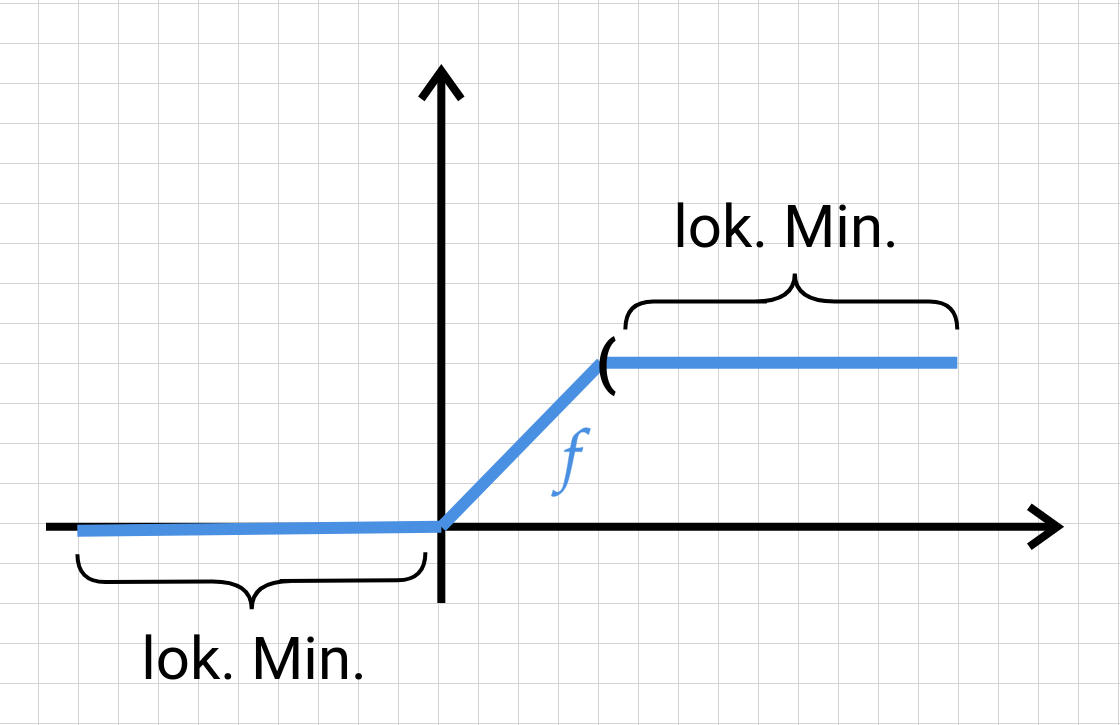
\includegraphics[width=0.5\textwidth]{pics/texplot3.png}
\end{center}
\caption{Quasikonvexe Funktion mit lokalem Minimum, dass zugleich globales Maximum ist}
\label{fig:quasikonvexeFunktion}
\end{figure}

\end{beispiel}

\begin{lemma}
\label{thm:quasikonvexlemma}
	Sei $X \subseteq \R^{n}$ konvex. Dann ist $f \colon X \rightarrow \R $ quasikonvex $\iff$
	$\forall c \in \R$ ist die Levelmenge 
	\[
	L_{c}(f) := \left\{ x \in X | f(x) \leq c \right\} 
	\] konvex.
\end{lemma}

\begin{proof}
\label{thm:quasikonvexlemmabeweis}
	Definitionen + Nachrechnen
\end{proof}

\begin{satz}
\label{thm:pseudoundquasikonvexität}
	Sei $X \subseteq \R^{n}$ offen, konvex und $f \colon X \rightarrow \R $ differenzierbar und pseudokonvex. Dann is $f$ auch quasikonvex.
	
	(Beweis ausgelassen)
\end{satz}

\begin{figure}[ht!]
	\begin{center}
		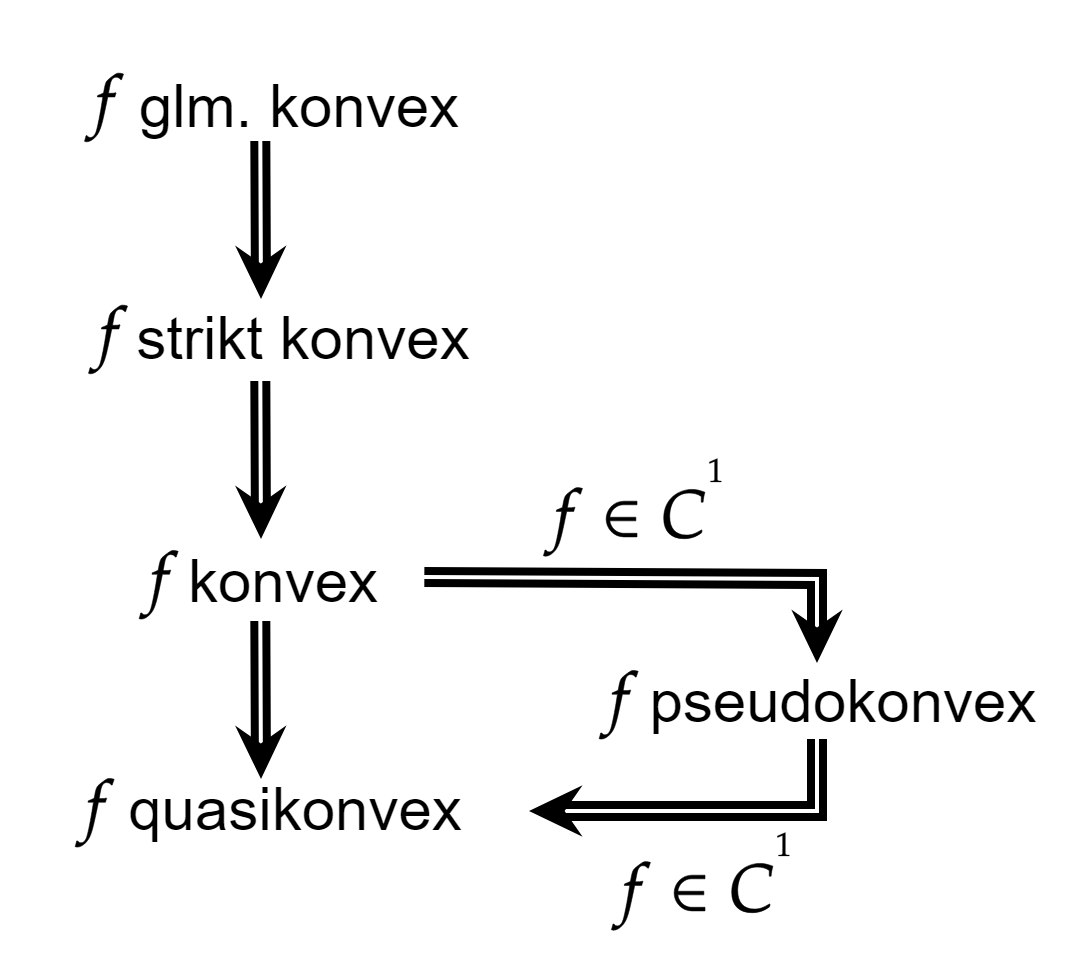
\includegraphics[width=0.5\textwidth]{pics/texplot4.png}
	\end{center}
	\caption{Übersicht über alle Arten von Konvexität und deren Zusammenhang}
	\label{fig:übersichtkonvex}
\end{figure}

\section{Monotone Funktionen}%
\label{sec:Monotone Funktionen}

\begin{definition}
\label{thm:monotonefunktionen}
	Sei $X \in \R^{n}$ und $F \colon X \rightarrow \R^{n}$. Dann heißt $F$
	\begin{itemize}
		\item \underline{monoton}, wenn gilt: $\forall x,y \in X$
			\[
				\left( F(x) - F(y) \right)^{T}(x-y) \geq 0	
			.\] 
		\item \underline{strikt monoton}, wenn gilt: $\forall x,y \in X$ mit $x \neq y$
			\[
				( F(x) - F(y) )^{T}(x-y) > 0	
			.\] 
		\item \underline{gleichmäßig monoton}, wenn gilt: $\exists \mu > 0, \forall x, y \in X$
			\[
				( F(x) - F(y) )^{T}(x-y) \geq \mu \norm{x-y} _{2}^{2}
			.\] 
	\end{itemize}
\end{definition}

\begin{beispiel}
\label{thm:beispielmonotonefunktionen1}
	Sei $f \colon \R \rightarrow \R $ monoton, d.h. $\forall x,y \in \R $
	\[
		(f(x)-f(y))^{T}(x-y) \geq 0
	.\]
	\begin{center}
			Fall 1: $x > y \implies f(x) \geq f(y)$

			Fall 2: $x < y \implies f(x) \leq f(y)$
	\end{center}

	Im Fall $n=1$ entspricht $F$ monoton der Eigenschaft, dass $F$ monoton \underline{wächst}.
\end{beispiel}

Es gilt
\[
F \text{ glm. mon. } \implies F \text{ strikt mon. } \implies F \text{ monoton}
.\] 

\begin{beispiel}
\label{thm:beispielmonotonefunktionen2}
	\begin{itemize}
		\item $f(x) \equiv c$ is monoton, aber nicht strikt monoton
		\item $f(x) = e^{x}$ is strikt monoton, aber nicht gleichmäßig monoton
		\item Sei $f(x) = Ax + b$ mit $ A \in \R^{n \times n}$. Dann gilt
			\begin{align*}
				f \text{ monoton } &\iff A \text{ positiv semidefinit} \\
				f \text{ strikt monoton } &\iff A \text{ positiv definit } \iff f \text{ glm. monoton}
			\end{align*}
			
	\end{itemize}
\end{beispiel}

\begin{satz}
\label{thm:monotonefunktionenäquivalenzen}
	Sei $X \subseteq \R^{n}$ nichtleer, konvex, affin und $f \colon X \rightarrow \R $ stetig diffbar. Dann gilt
	\begin{enumerate}[label=(\alph{enumi})]
		\item $f$ ist konvex $\iff$ $F(x):= \nabla f(x)$ monoton
		\item $f$ ist strikt konvex $\iff$ $\nabla f$ strikt monoton
		\item $f$ ist gleichmäßig konvex $\iff$ $\nabla f$ glm. monoton
	\end{enumerate}
\end{satz}

\begin{proof}
\label{thm:monotonefunktionenäquivalenzenbeweis}
\begin{itemize}
	\item (c)
		\begin{itemize}
			\item "$\implies$": Sei $f$ gleichmäßig konvex. Dann gilt für alle $x,y \in X$ und $\mu>0$ fest:
		\begin{align*}
			f(x) - f(y) &\geq \nabla f(y)^{T}(x-y) + \mu \norm{x-y} _{2}^2 \\
			f(y) - f(x) &\geq \nabla f(x)^{T}(y-x) + \mu \norm{y-x} _{2}^2
		\end{align*}
		Addieren der Ungleichung ergibt
		\[
			0 \geq (\nabla f(y) - \nabla f(x))^{T}(x-y) + 2 \mu \norm{x-y} _{2}^2
		.\] 
		Also ist $\nabla f$ gleichmäßig monoton

			\item "$\Longleftarrow$": Sei $\nabla f$ glm. monoton, d.h. es gibt $\mu>0$ mit 
				\[
					\forall x,y \in X : (\nabla f(x) - \nabla f(y))^{T}(x-y) \geq \mu \norm{x-y} _{2}^2
				.\] 
				Seien $x,y \in X$ beliebig. Dann gibt es nach dem Mittelwertsatz ein $c \in(0,1)$ mit
				\[
					\label{eq:mon1}\tag{$\ast$}
					f(x) -f(y) = \nabla f(y + c(x-y))^{T}(x-y)
				.\] 
				Wegen der glm. Monotonie gilt
				\[
					\label{eq:mon2}\tag{$\ast\ast$}
					c(\nabla f(y+c(x-y))-\nabla f(y))^{T}(x-y) \geq c^2 \norm{x-y} _{2}^2
				.\] 
				Also folgt:
				\begin{align*}
					f(x)-f(y) \overset{\href{eq:mon1}{(\ast)}}&{=} \nabla  f(y+ c(x-y))^{T}(x-y) \\
															  & \geq \nabla  f(y)^{T}(x-y) + \underbrace{\mu c}_{=:\tilde{\mu}(c)} \norm{ x-y } _{2}^2 
				\end{align*}

				Problem : $c \in (0,1)$ kann beliebig klein werden:

				\underline{Lösungsansatz:} 
				% TODO : Bild 1 einfügen

				Wähle $ m \in \N$ beliebig, definiere
				\begin{align*}
					t_{k}&:= \frac{k}{m+1} \text{ für } k=0, \ldots, m+1 \\
					x_{k}&:= y + t_{k}(x-y)
				\end{align*}
				Der Mittelwertsatz impliziert $\forall k=0, \ldots, m ~\exists c_{k} \in(t_{k}, t_{k+1})$:
				\[
					f(x_{k+1}) -f(x_{k}) = \nabla  f(y + c_{k}(x-y))^{T}\underbrace{x_{k+1}- x_{k}}_{= (t_{k+1}- t_{k})(x-y)} 
				.\] 
				Damit folgt:
				\begin{align*}
					f(x)-f(y) &= f(x_{m+1}) - f(x_{0}) \\
							  &= \sum_{k=0}^{m}{f(x_{k+1}) - f(x_{k})} \\
							  &= \sum_{k=0}^{m}{(t_{k+1}-t_{k})\nabla f(y+c_{k}(x-y))^{T}(x-y)} \\
							  &+ \sum_{k=0}^{m}{(\nabla f(y) - \nabla f(x))^{T}\underbrace{t_{k+1}-t_{k})(x-y)}_{= x_{k+1}-x_{k}}} \\
							  &= \nabla f(y)^{T}(x-y) \\
							  &+ \sum_{k=0}^{m}{(t_{k+1}-t_{k})\left[ \nabla f(y+c_{k}(x-y)) - \nabla f(y) \right] ^{T} \underbrace{(x-y)}_{=\frac{1}{c_{k}}\left[ y + c_{k}(x-y) - y \right] } } \\
							  &\geq \nabla f(y)^{T}(x-y) \\
							  &+ \sum_{k=0}^{m}{\frac{t_{k+1}- t_{k}}{c_{k}} \mu c_{k}^2 \norm{x-y} _{2}^2} \\
							  &= \nabla f(y)^{T}(x-y) + \frac{\mu \norm{x-y} _{2}}{m+1} \underbrace{\sum_{k=0}^{m}{\underbrace{c_{k}}_{\geq t_{k}= \frac{k}{m+1}} }}_{\geq \frac{m}{2}}   \\
							  &\geq \nabla f(y)^{T}(x-y) + \mu  \norm{x-y} ^2 \cdot \underbrace{\frac{m}{2(m+1)}}_{\rightarrow \frac{1}{2} \text{ für } m \rightarrow \infty} 
				\end{align*}
		\end{itemize}

\item (a): funktioniert wie (c) mit $\mu =0$ und ohne Intervallaufteilung. 
\item (b): funktioniert wie (c) mit $\mu =0$ mit strikten Ungleichungen und ohne Intervallaufteilung.
\end{itemize}
\end{proof}

\begin{satz}
\label{thm:monotonefunktionenunddefinitheit}
	Sei $X \subseteq \R^{n}$ nichtleer, affin, konvex und $F \colon X \rightarrow \R^{n} $ stetig diffbar. Dann gilt:
	\begin{enumerate}[label=(\alph{enumi})]
		\item $F$ monoton $\iff$ $\forall x \in X$ : $F(x)$ positiv semidefinit, d.h.
			\[
				d^{T}F'(x)d \geq 0 \quad \forall d \in \R^{n}
			.\] 
		\item $F$ strikt monoton $\Longleftarrow$ $\forall x \in X$ : $F'(x)$ ist positiv definit, d.h.
			\[
				d^{T}F'(x)d >  \quad \forall d \in \R^{n}\setminus \left\{ 0 \right\} 
			.\] 
		\item $F$ glm. monoton $\iff$ $\exists \mu > 0 ~ \forall x \in X$ : $F'$ glm. positiv definit
			\[
				d^{T} F'(x) d \geq \mu \norm{d} ^2 \quad \forall d \in \R^{n}
			.\]
	\end{enumerate}
\end{satz}

\begin{proof}
\label{thm:monotonefunktionenunddefinitheitbeweis}
\begin{itemize}
	\item (c)
		\begin{itemize}
			\item "$\implies$" : Sei $F$ glm. monoton, d.h. $\exists \mu > 0 ~ \forall x,y \in X$ : 
				\[
				(F(x)-F(y))^{T}(x-y) \geq \mu \norm{x-y} _{2}^2
				.\] 
				Sei $x \in X, d \in \R^{n}$ beliebig. Dann gilt
				\begin{align*}
					d^{T} \underbrace{F'(x)d}_{=F'(x;d)} &= \lim_{t \downarrow 0}  \frac{td^{T}(F(x+td) - F(x))}{t^2} \\
														 &\geq \lim_{t \downarrow 0}  \frac{\mu  t^2 \norm{d} ^2}{t^2} = \mu  \norm{d} ^2
				\end{align*}
				Das bedeutet $F'$ ist glm. positiv definit.

			\item "$\Longleftarrow$" : Sei $F'$ glm. positiv definit, d.h. $\exists \mu >0 ~ \forall x \in X ~ \forall d \in \R^{n}$ : 
				\[
					d^{T}F'(x)d \geq \mu \norm{d} _{2}^2
				.\] 
				Seien $x,y \in X$ beliebig. Dann gilt
				\begin{align*}
					(F(x)-F(y))^{T}(x-y) &= \int_{0}^{1} \underbrace{(x-y)^{T}F'(y+ \tau (x-y))(x-y)}_{\geq \mu \norm{x-y} _{2}^2} \d \tau \\
										 &\geq \mu  \norm{x-y} _{2}^2
				\end{align*}
		\end{itemize}
	\item (a) funktioniert wie (c) mit $\mu =0$
	\item (c) "$\Longleftarrow$" wie (c) mit $\mu =0$ und $F'$ positiv definit

		["$\implies$" geht kaputt wegen $\lim\limits_{t \downarrow 0}$ ]
\end{itemize}
\end{proof}

\begin{folgerung}
\label{thm:monotonefunktionenkonvexefunktionenfolgerung}
% TODO : Flussdiagramm
\end{folgerung}

\begin{definition}
\label{thm:pseudoquasimonoton}
	Sei $X \subseteq \R^{n}$ und $F \colon X \rightarrow \R^{n} $
	\begin{enumerate}[label=(\alph{enumi})]
		\item  $F$ heißt \underline{pseudomonoton} $\iff$ $\forall x,y \in X$ : 
			\[
				F(y)^{T}(x-y) \geq 0 \implies F(x)^{T}(x-y) \geq 0
			.\] 
		\item $F$ heißt \underline{quasimonoton} $\iff$ $\forall x,y \in X$ :
			\[
				\min \left\{ F(x)^{T}(x-y), F(y)^{T}(y-x) \right\} \leq 0
			.\] 
	\end{enumerate}

	Man kann zeigen:
	\begin{itemize}
		\item $f$ pseudokonvex $\iff$ $\nabla f$ pseudomonoton
		\item Ist $F$ pseudomonoton, so gilt $\forall x,y \in X$ :
			\[
				F(y)^{T} (x-y) > 0 \implies F(x)^{T} (x-y) > 0
			.\] 
		\item Ist $F$ quasimonoton und diffbar, so ist $\nabla F$ quasimonoton
	\end{itemize}
	
\end{definition}
